\documentclass{article}
\usepackage{amsmath}
\usepackage{booktabs}
\usepackage{caption}
\usepackage{float}
\usepackage{amsmath}
\usepackage{amssymb}
\usepackage{physics}
\usepackage{graphicx}
\usepackage[margin=0.7in]{geometry}
\usepackage{apacite}
\title{Personalized Movie Recommendation using Probabilistic Matrix Factorization and Bayesian Reasoning}

\begin{document}

\maketitle

\section{Introduction}
Finding the perfect movie is often harder than it seems. With so many options and platforms, it is easy to get lost scrolling endlessly through suggestions that miss the mark. Browsing IMDB or relying on generic recommendation lists can feel time-consuming and unsatisfying. Most current movie recommendation systems rely on surface-level preferences, like genre or popularity, or collaborative filtering, which compares users' habits without truly understanding individual tastes. In this project, our aim is to create a smarter solution by using probabilistic matrix factorization to build a recommendation system that learns from users' unique preferences and behaviors, offering more personalized and insightful movie suggestions.

Our movie recommendation system uses a small set of user ratings to predict films that best align with a user's personal tastes. The system is built on a probabilistic matrix factorization (PMF) approach, which models user preferences and movie characteristics in a lower-dimensional space.

By learning latent factors from user ratings, the system identifies patterns that relate users to movies they are likely to enjoy. When a new user provides their ratings, the system adjusts these factors to reflect their specific preferences, predicting how they might rate other movies they have not seen yet. This allows us to recommend films that are most likely to resonate with the user based on these learned relationships.

The movies are ranked according to predicted ratings, prioritizing recommendations that are most likely to satisfy the user. Finally, the system presents movie recommendations according to user-defined filters, such as genres and years.

\section{Data Processing}
In our data processing pipeline, we begin by downloading the MovieLens ml-latest-small dataset to train and evaluate our recommendation system (https://grouplens.org/datasets/movielens/). This dataset provides 100K user ratings from 600 users for 9000 movies, along with additional information such as genre, IMDB ratings, and tags.

The next step is to load the raw movie rating data and metadata into the data frames. The ratings dataset is then filtered to remove users and movies that have insufficient ratings, based on a user-defined threshold. This ensures that enough data exist for a user or movie for the model to learn their feature vector.

After this, the filtered ratings data is transformed into a rating matrix where each row represents a user and each column represents a movie. The values in this matrix correspond to the user's ratings, with missing entries for movies that haven’t been rated by a particular user.

We then split this rating matrix into training and testing sets by users, with 80\% of the data used for training and the remaining 20\% for testing. Finally, key statistics such as sparsity and the dimensions of the training and test matrices are displayed, and the processed data is saved for later stages in model development.


\section{Probabilistic Matrix Factorization}

Given a sparse ratings matrix $R$, we want to be able to estimate the missing data in the matrix. A way of doing this is through Probabilistic Matrix Factorization (PMF) \cite{salakhutdinov2007}.

Suppose we have $M$ movies and $N$ users as well as rating values between 1 and 5. We now let $R_ {ij}$ represent user $i$'s rating of movie $j$. Let $U \in R^{D \times N}$ be the latent user feature matrix and let $V \in R^{D \times M}$ bet the latent movie feature matrix, with column-vectors $U_i$ representing user-specific and $V_j$ representing movie-specific latent feature vectors respectively. The idea is that we want to find $U$ and $V$ such that
\begin{equation}
    R \approx UV^T.
\end{equation}

We assume that
\begin{equation}
    R_{ij} = [U_iV_j^T + \epsilon_{ij}]^{I_{ij}}, \;\;\; \epsilon_{ij} \sim \mathcal{N}(0, \sigma^2),
\end{equation}
where $I_{ij}$ is the indicator function which will be equal to 1 if user $i$ rated movie $j$ and equal to 0 otherwise. The choice of D reflects the number of latent factors one wishes to capture in the model.

The key idea is that a movie rating is a dot product of two vectors, one representing the user's preferences and one representing the movie's attributes in some space. The PMF framework assumes that the rating matrix $R$ can be approximated by a product of two lower-dimensional matrices $U$ and $V$.

Define the conditional distribution over the observed ratings as
\begin{equation}
    p(R \mid U,V, \sigma^2)= \prod_{i=1}^N \prod_{j=1}^M \left[ \mathcal{N}(R_{ij} \mid U_i^TV_j, \sigma^2) \right]^{I_{ij}}
\end{equation}
where $\mathcal{N}(x \mid \mu, \sigma^2)$ is the usual probability density function of the Gaussian distribution with mean $\mu$ and variance $\sigma^2$.

The user and movie feature vectors are given zero-mean spherical Gaussian priors:
\begin{equation}
    p(U \mid \sigma^2_U) = \prod_{i=1}^N\mathcal{N}(U_i \mid 0, \sigma_U^2 \textbf{I})
\end{equation}
\begin{equation}
    p(V \mid \sigma^2_V) = \prod_{j=1}^M\mathcal{N}(V_j \mid 0, \sigma_V^2 \textbf{I})
\end{equation}

We will now derive the log of the posterior distribution over user and movie features.
We have that
\begin{equation}
    P(U,V \mid R, \sigma^2, \sigma_U^2, \sigma_V^2) = \frac{P(U \mid \sigma_U^2)P(V \mid \sigma_V^2)P(R \mid U,V, \sigma^2)}{P(R)},
\end{equation}

and that:
\begin{equation}
    P(U \mid \sigma_U^2) = \prod_{i=1}^N \prod_{k=1}^D \frac{1}{\sqrt{2\pi} \sigma_U}e^{-\frac{U_i^2 k}{2 \sigma_U^2}}
\end{equation}
\begin{equation}
    P(V \mid \sigma_V^2) = \prod_{j=1}^M \prod_{k=1}^D \frac{1}{\sqrt{2\pi} \sigma_V}e^{-\frac{V_j^2 k}{2 \sigma_V^2}}
\end{equation}
\begin{equation}
    P(R \mid U,V, \sigma^2) = \prod_{i=1}^N \prod_{j=1}^M \frac{1}{\sqrt{2\pi}\sigma}e^{- \frac{1}{2 \sigma^2} [(R_{ij}-U_iV_j^T)^2]^{I_{ij}}}.
\end{equation}
$P(R)$ is constant.

Thus the log probability of the posterior is:
\begin{align}
    \ln P(U, V \mid R, \sigma^2, \sigma_U^2, \sigma_V^2) & = \ln P(U \mid \sigma_U^2) + \ln P(V \mid \sigma_V^2)                                                               \\
                                                         & + \ln P(R \mid U,V, \sigma^2) - \ln P(R) \nonumber                                                                  \\
                                                         & = \sum_{i=1}^N \sum_{k=1}^D (- \frac{U_i^2k}{2 \sigma_U^2} - \ln \sqrt{2\pi} \sigma_U)                              \\
                                                         & + \sum_{j=1}^M \sum_{k=1}^D (- \frac{V_j^2k}{2 \sigma_V^2} - \ln \sqrt{2\pi} \sigma_V) \nonumber                    \\
                                                         & + \sum_{i=1}^N \sum_{j=1}^M (- \frac{1}{2\sigma^2}[(R_{ij}-U_iV_j^T)^2]^{I_{ij}} - \ln \sqrt{2\pi}\sigma) \nonumber \\
                                                         & - P(R) \nonumber                                                                                                    \\
                                                         & = -\frac{1}{2\sigma^2} \sum_{i=1}^N \sum_{j=1}^M [(R_{ij} - U_iV_j^T)^2]^{I_{ij}}                                   \\
                                                         & - \frac{1}{2\sigma_U^2} \sum_{i=1}^N U_iU_i - \frac{1}{2 \sigma_V^2} \sum_{j=1}^M V_jV_j \nonumber                  \\
                                                         & - MN \ln \sigma - ND \ln \sigma_U - MD \ln \sigma_V + C \nonumber
\end{align}


Maximizing $\ln P(U, V \mid R, \sigma^2, \sigma_U^2, \sigma_V^2)$ is equal to minimizing the following:
\begin{equation}
    L = \frac{1}{2} \sum_{i=1}^N \sum_{j=1}^M [(R_{ij}-U_iV_J^T)^2]^{I_{ij}}
    + \frac{\lambda_U}{2} \sum_{i=1}^N||U_i||_{F}^2
    + \frac{\lambda_V}{2} \sum_{j=1}^M||V_j||_{F}^2.
\end{equation}
Here $\lambda_U = \frac{\sigma^2}{\sigma_U^2}$ and $\lambda_V = \frac{\sigma^2}{\sigma_U^2}{}$ are hyper-parameters and $||\cdot||_{F}$ indicates the Frobenius norm.

The loss function has the following derivatives:
\begin{equation}
    \frac{\partial L}{\partial U_i} = \sum_{j=1}^M[U_iV_j^T-R_{ij}]^{I_{ij}}V_j + \lambda_UU_i = [\hat{R}_i-R_i]^{I_{ij}}V + \lambda_UU_i
\end{equation}
\begin{equation}
    \frac{\partial L}{\partial V_j} = \sum_{i=1}^N[U_iV_j^T-R_{ij}]^{I_{ij}}U_i + \lambda_VV_j = ([\hat{R}_i-R_i]^{I_{ij}})^TU + \lambda_VV_j.
\end{equation}

These are used for gradient descent to obtain $U$ and $V$ that minimize the loss by iteratively updating:
\begin{equation}
    U \gets U - \eta([\hat{R}-R]^{I_{ij}}V + \lambda_UU)
\end{equation}
\begin{equation}
    V \gets V - \eta(([\hat{R}-R]^{I_{ij}})^TU + \lambda_VV)
\end{equation}
where $\eta$ is the learning rate to be chosen. U and V are initialized as normally distributed with mean $\mu=0$ and standard deviation $\sigma = \frac{1}{D}$ before performing gradient descent.

There are multiple hyper-parameters to decide: $\lambda_U$, $\lambda_V$, $D$ and $\eta$. Especially D is of interest, as it is the number of latent features captured. If D is too small it might fail to capture the nuances of user preferences and movie features, where as if it is too large it might overfit (even though the Gaussian priors help).


\section{Inference Using Fitted Model}
The general procedure of using the fitted matrices $U$ and $V$ to provide recommendations is as follows:
\begin{enumerate}
    \item The user provide their own rating for some movies.
    \item The predictor learns the preference vector of the user and predicts ratings for other movies using the fitted model and given ratings.
    \item The predictor classifies movies by predicted ratings into movies to recommend if the predicted ratings fall within a user-defined rating range.
    \item To finalize the results, the predictor sorts the recommendations and optionally filters by user-defined genres and years.
\end{enumerate}

\subsection{Partial PMF}
To learn the preference vector of the new user $\vec{u}$ we make the following assumptions:
\begin{align}
    \vec{r}  & = V \vec{u} + \epsilon    \\
    \vec{u}  & \sim N^D(0, \sigma_u^2 I) \\
    \epsilon & \sim N(0, \sigma^2)       \\
    \vec{u}  & \perp V
\end{align}

Instead of using the complete PMF, we use partial PMF to learn the preference vector of new user, by holding the matrix $V$ from previous section fixed \cite{salakhutdinov2007}. Given ratings $\vec{r}$ and $V$, we maximize:
\begin{align}
    \ln{P(\vec{u} | V, \vec{r})} & = \ln{P(\vec{u})} + \ln{P(\vec{r} | \vec{u}, V)} - \ln{P(\vec{r} | V)}                                               \\
                                 & = -\frac{1}{2 \sigma_u^2} \vec{u}^2 - \frac{1}{2 \sigma^2} \sum_{j=1}^m \mathbb{I}_j (\vec{V_j} \vec{u} - r_j)^2 + c
\end{align}

Let $L = -\ln{P(\vec{u} | V, \vec{r})}$, we minimize:
\begin{align}
    L                         & = \frac{1}{2 \sigma^2} \sum_{j=1}^m \mathbb{I}_j (\vec{V_j} \vec{u} - r_j)^2 + \frac{1}{2 \sigma_u^2} \vec{u}^2 \\
    \frac{\dd L}{\dd \vec{u}} & = ((V \vec{u} - \vec{r}) \odot \vec{\mathbb{I}}) V + \lambda \vec{u}
\end{align}
where $\odot$ represent element-wise operation, $\vec{\mathbb{I}}$ is the indicator vector for the new user, and $\lambda = \sigma^2 / \sigma_U^2$.

Since we cannot analytically solve the nullcline equation, we use gradient descent to learn feature vector of the new user:
\begin{align}
    \vec{u} & \leftarrow \vec{u} - \eta \left(((V \vec{u} - \vec{r}) \odot \vec{\mathbb{I}}) V + \lambda \vec{u}\right)
\end{align}

With the user preference vector, we can predict the user's ratings for other movies:
\begin{align}
    \hat{r} & = V \vec{u}
\end{align}

\subsection{Estimating Empirical Variance of Prediction}
In addition to predicted ratings, we also want to know the standard deviation of our predictions, which reflects the confidence level the predictor has on the ratings. We cannot simply use $\sigma^2$ and $\sigma_U^2$ from previous assumptions, because they only enter the model through $\lambda_U = \sigma^2 / \sigma_U^2$ as ratio. We do not know their actual values. In fact, $\sigma^2$, $\sigma_U^2$ or $\sigma_V^2$ can be different between different elements in $U$ and $V$, as long as they have the same ratio. In addition to these considerations, to reflect the impact of missingness in some of training data, we need to obtain the empirical variance and covariance matrix for our parameters to estimate standard deviation for predicted ratings.

Before estimating covariance matrices for parameters, we need to make additional assumptions for simplicity:
\begin{align}
    \vec{u_i} & \perp \vec{u_j},\: \forall \vec{u_i}, \vec{u_j}, i \ne j \in U \\
    \vec{v_i} & \perp \vec{v_j},\: \forall \vec{v_i}, \vec{v_j}, i \ne j \in V \\
    U         & \perp V
\end{align}

We can approximate the covariance matrix of parameters using the inverse of Hessian matrix of objective function, which is the loss function, with regard to parameters \cite{baker2021}:
\begin{align}
    \operatorname{Cov}(\vec{x}) & \approx H^{-1}(L, \vec{x}) = \left(\frac{\partial^2 L}{\partial \vec{x}^2}\right)^{-1}
\end{align}

In this way, covariance matrix for $\vec{v_j} \in V$ can be estimated:
\begin{align}
    L                             & = -\ln{P(U, V | R)} = \frac{1}{2} \sum_{i,j} (R_{ij} - \vec{u_i} \cdot \vec{v_j})^2 \mathbb{I}_{ij} + \frac{\lambda_U}{2} \sum_i \vec{u_i}^2 + \frac{\lambda_V}{2} \sum_j \vec{v_j}^2 \\
    \operatorname{Cov}(\vec{v_j}) & \approx H^{-1}(L, \vec{v_j}) = \left(\frac{\partial^2 L}{\partial \vec{v_j}^2}\right)^{-1} = \left(U^\top (U \odot \vec{\mathbb{I}_{:j}}) + \lambda_V I\right)^{-1}
\end{align}

and the covariance matrix for new user $\vec{u}$:
\begin{align}
    L                           & = \frac{1}{2 \sigma^2} \sum_{j=1}^m \mathbb{I}_j (\vec{V_j} \vec{u} - r_j)^2 + \frac{1}{2 \sigma_u^2} \vec{u}^2                                          \\
    \operatorname{Cov}(\vec{u}) & \approx H^{-1}(L, \vec{u}) = \left(\frac{\partial^2 L}{\partial \vec{u}^2}\right)^{-1} = \left(V^\top (V \odot \vec{\mathbb{I}}) + \lambda I\right)^{-1}
\end{align}

For simplicity of notation, let $\vec{v} = \vec{V_j}$, $r = r_j$. Predicted rating for movie $M_j$:
\begin{align}
    \hat{r}                       & = \vec{u} \cdot \vec{v} = \sum_{k=1}^D u_k v_k                                                                                                             \\
    \operatorname{Var}{(\hat{r})} & = \sum_{k=1}^D \operatorname{Var}{(u_k v_k)} + \sum_{i,j:\:i \ne j} \operatorname{Cov}(u_i v_i, u_j v_j) = \sum_{i,j} \operatorname{Cov}(u_i v_i, u_j v_j)
\end{align}

Expand the covariance:
\begin{align}
    \operatorname{Cov}(u_i v_i, u_j v_j) & = \operatorname{E}(u_i v_i u_j v_j) - \operatorname{E}(u_i v_i) \operatorname{E}(u_j v_j)                                     \\
                                         & = \operatorname{E}(u_i v_i u_j v_j) - \operatorname{E}(u_i) \operatorname{E}(v_i) \operatorname{E}(u_j) \operatorname{E}(v_j)
\end{align}

Let $\bar{x}$ represent the expectation of random variable $x$. In our case, $\bar{u_i}$ is the actual value of $u_i$ and $\bar{v_i}$ is the actual value of $v_i$. Using Isserlis' rule:
\begin{align}
      & \operatorname{E}[(u_i - \bar{u_i}) (v_i - \bar{v_i}) (u_j - \bar{u_j}) (v_j - \bar{v_j})]                                                                                                                                           \\
    = & \operatorname{Cov}[(u_i - \bar{u_i}), (u_j - \bar{u_j})] \operatorname{Cov}[(u_i - \bar{u_i}), (v_j - \bar{v_j})] \operatorname{Cov}[(v_i - \bar{v_i}), (u_j - \bar{u_j})] \operatorname{Cov}[(v_i - \bar{v_i}), (v_j - \bar{v_j})] \\
    = & \operatorname{Cov}[u_i, u_j] \operatorname{Cov}[v_i, v_j]
\end{align}

Let $\tilde{x} = x - \bar{x}$ represent 0-centered random variable. Completing the last piece:
\begin{align}
    \operatorname{E}(u_i v_i u_j v_j)                & = \operatorname{E}[(\bar{u_i} + \tilde{u_i}) (\bar{v_i} + \tilde{v_i}) (\bar{u_j} + \tilde{u_j}) (\bar{v_j} + \tilde{v_j})]                                                                                                                         \\
                                                     & = \bar{u_i} \bar{v_i} \bar{u_j} \bar{v_j} + (\bar{v_i} \bar{v_j}) \operatorname{E}(\tilde{u_i}, \tilde{u_j}) + (\bar{u_i} \bar{u_j}) \operatorname{E}(\tilde{v_i}, \tilde{v_j}) + \operatorname{E}(\tilde{u_i} \tilde{u_j} \tilde{v_i} \tilde{v_j}) \\
                                                     & = \bar{u_i} \bar{v_i} \bar{u_j} \bar{v_j} + (\bar{v_i} \bar{v_j}) \operatorname{Cov}(u_i, u_j) + (\bar{u_i} \bar{u_j}) \operatorname{Cov}(v_i, v_j) + \operatorname{Cov}(u_i, u_j) \operatorname{Cov}(v_i, v_j)                                     \\
    \Rightarrow \operatorname{Cov}(u_i v_i, u_j v_j) & = (\bar{v_i} \bar{v_j}) \operatorname{Cov}(u_i, u_j) + (\bar{u_i} \bar{u_j}) \operatorname{Cov}(v_i, v_j) + \operatorname{Cov}(u_i, u_j) \operatorname{Cov}(v_i, v_j)
\end{align}

Therefore, the variance is:
\begin{align}
    \operatorname{Var}{(r)} & = \sum_{i,j} \operatorname{Cov}(u_i v_i, u_j v_j)                                                                                                                                             \\
                            & = \sum_{i,j} \left[(\bar{v_i} \bar{v_j}) \operatorname{Cov}(u_i, u_j) + (\bar{u_i} \bar{u_j}) \operatorname{Cov}(v_i, v_j) + \operatorname{Cov}(u_i, u_j) \operatorname{Cov}(v_i, v_j)\right]
\end{align}

\section{Experiment and Analysis}

\subsection{Experiment Settings}

To evaluate the performance of our movie recommendation model, we conducted experiments on a test dataset containing user ratings for movies. The model was evaluated under different input sizes (proportion of observed ratings used as input) and compared against a random control baseline. The metrics used for evaluation were:

\begin{itemize}
    \item Precision ($P$):
          Proportion of correct recommendations out of the total recommendations. A recommendation is considered correct if the actual rating of the movie falls within the specified rating range.
          \[ P = \frac{\text{True Positives}}{\text{True Positives} + \text{False Positives}} \]

    \item Recall ($R$): Proportion of relevant movies that are recommended, where a relevant movie is one that the user has rated within the specified rating range.
          It is defined as:
          \[ R = \frac{\text{True Positives}}{\text{True Positives} + \text{False Negatives}} \]

    \item F1-Score ($F_1$): Harmonic mean of Precision and Recall. It is calculated as:
          \[ F_1 = 2 \cdot \frac{P \cdot R}{P + R} \]

    \item Mean Absolute Error (MAE): Average absolute difference between predicted and actual ratings. It is calculated as:
          \[ \text{MAE} = \frac{1}{n} \sum_{i=1}^n | \text{predicted rating}_i - \text{actual rating}_i | \]
\end{itemize}

For the experiments, we varied the \texttt{input\_size} parameter, which determines the fraction of observed ratings used for generating recommendations. The model's performance was compared against a random recommendation baseline to demonstrate its effectiveness.

\subsection{Selection of Hyper-Parameters}
We tested different values of $D$, meaning the number of latent features, to see how they influence the MAE. On figure \ref{fig:LatentPlot} the results can be seen. It seems that the optimal choice of $D$ for accuracy is somewhere around 30.

\begin{figure}[H]
    \centering
    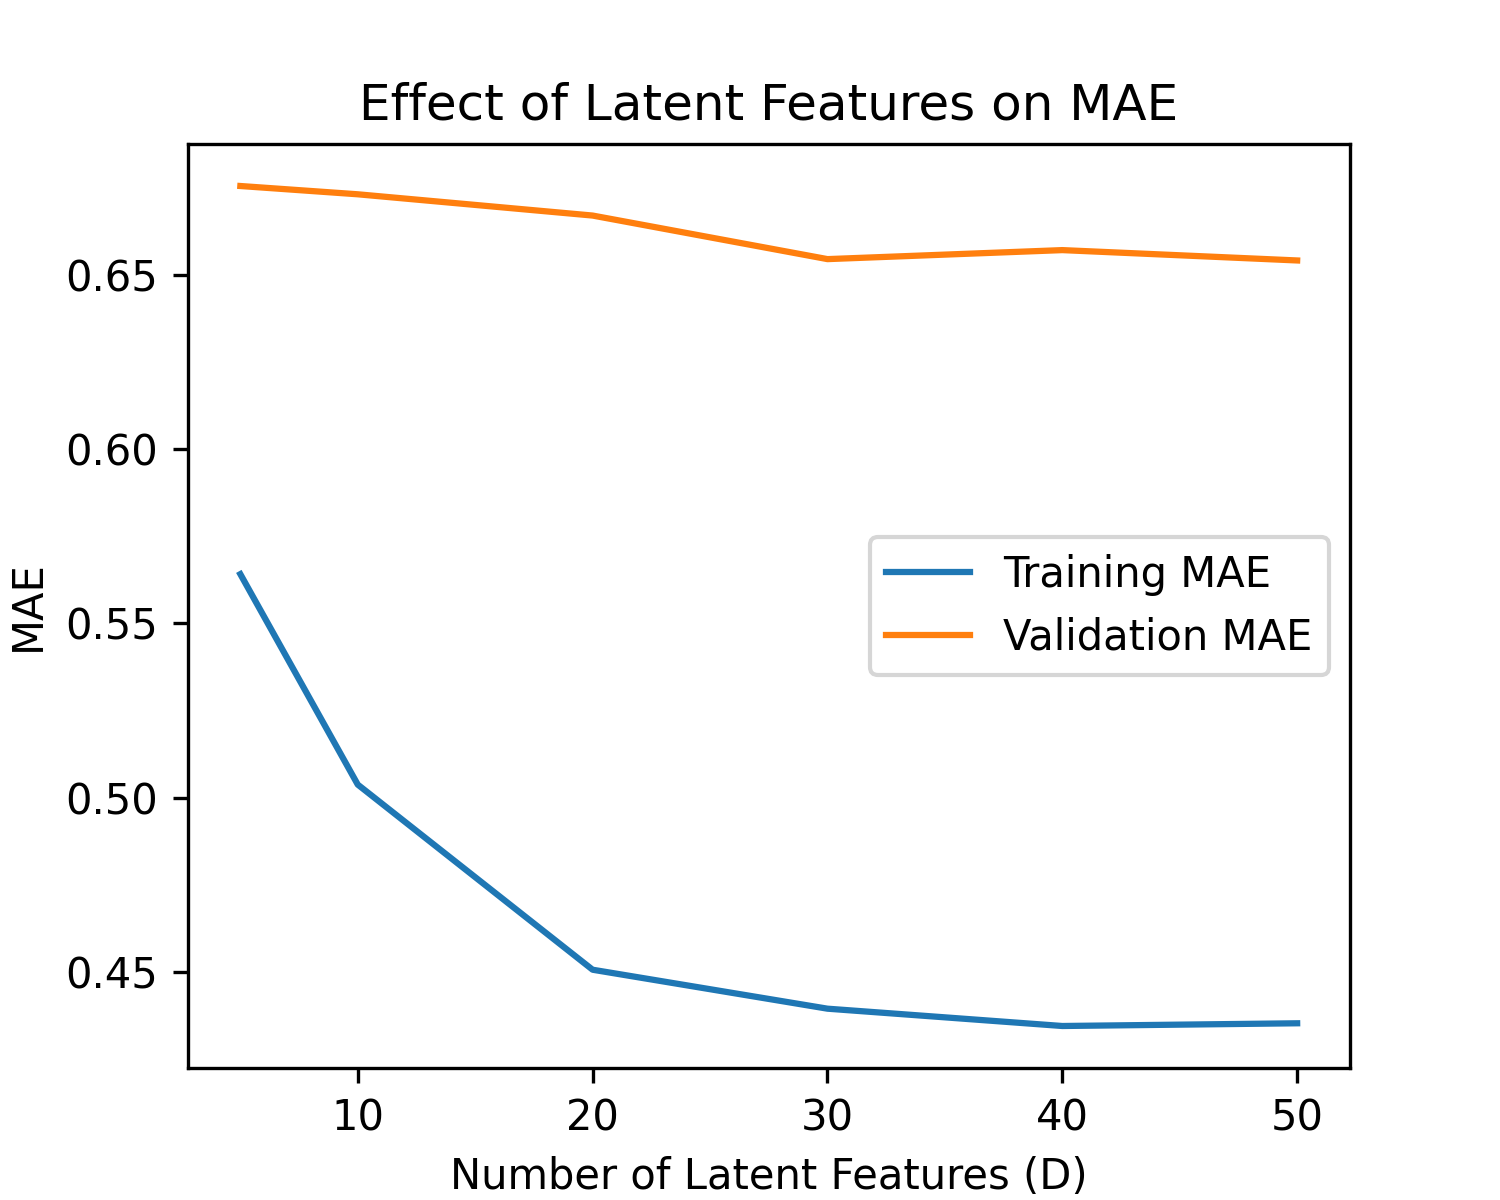
\includegraphics[scale = 0.7]{latent_features_MAE.png}
    \caption{}
    \label{fig:LatentPlot}
\end{figure}

We tested out how the loss changes as a function of the number of epochs in training. For this test we used the following hyper parameters:
$$\lambda_U = 1 \;\;\;\; \lambda_V = 1 \;\;\;\; \eta=10^{-4} \;\;\;\; D=25$$
We did a relatively simple search and found that those parameters performed well.

The result of the test can be seen in figure \ref{fig:LossPlot}. It is seen that the validation loss quite quickly somewhat stagnates, where as the training loss keeps lowering quicker.

\begin{figure}[H]
    \centering
    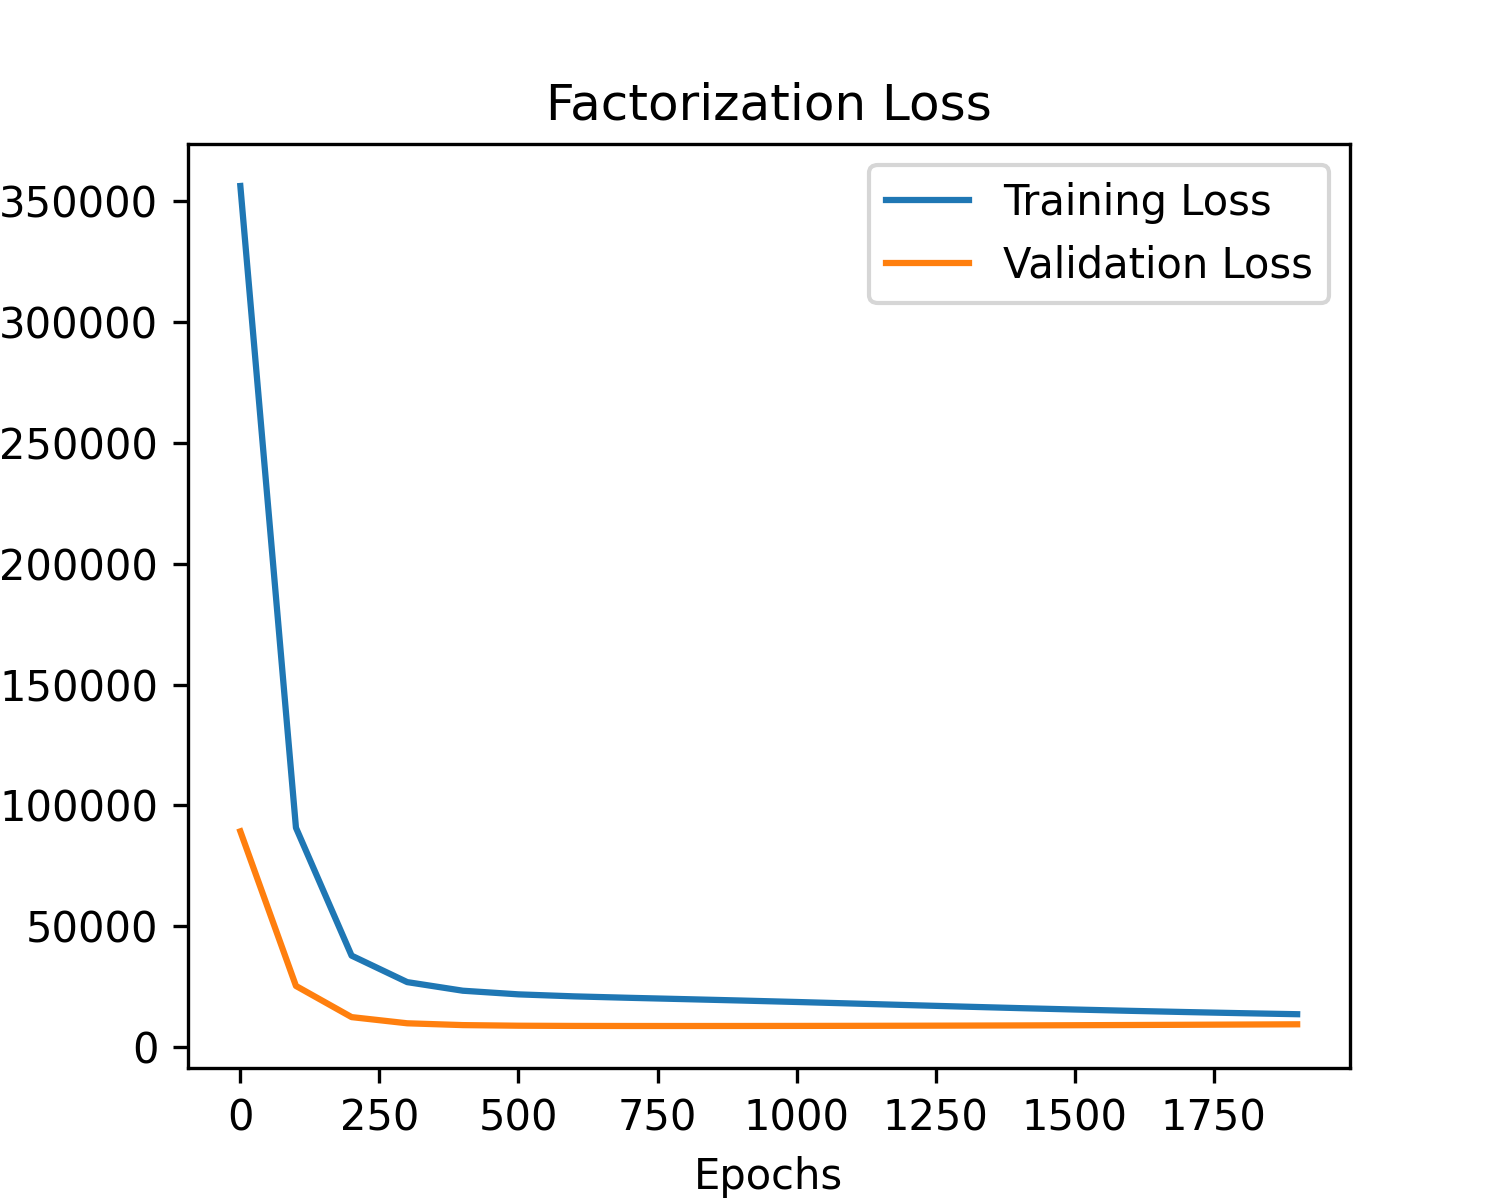
\includegraphics[scale = 0.7]{loss.png}
    \caption{}
    \label{fig:LossPlot}
\end{figure}

\subsection{Performances of Model and Predictor}
Using these methods, we implemented the inference module `infer.py'. The model in combination with the predictor displayed high performance with overall precision 0.87 and recall 0.73, respectively, compared to 0.62 and 0.50 in baseline (Figure \ref{fig:inference}A-D), which randomly picks movies as recommendations. By providing ratings to some movies, we obtained recommendations from our system, which is, subjectively, very accurate (Figure \ref{fig:inference}E-F). The distributions of predicted ratings and standard deviations are also shown, in which standard deviations range from 1.5 to 4.5, within a reasonable range (Figure \ref{fig:inference}G-H). Notably, the standard deviation also helped us in choosing appropriate $D$, the number of latent features in $U$ and $V$. Previously, we used $D=100$, yielding low loss on training data but also suboptimal precision on test data. We observed that the standard deviation for ratings could get as large as 50 since large amount of latent features amounts to large variation in predictions. With this observation we lowered $D$ to 25, achieving our current performance.

\begin{figure}
    \centering
    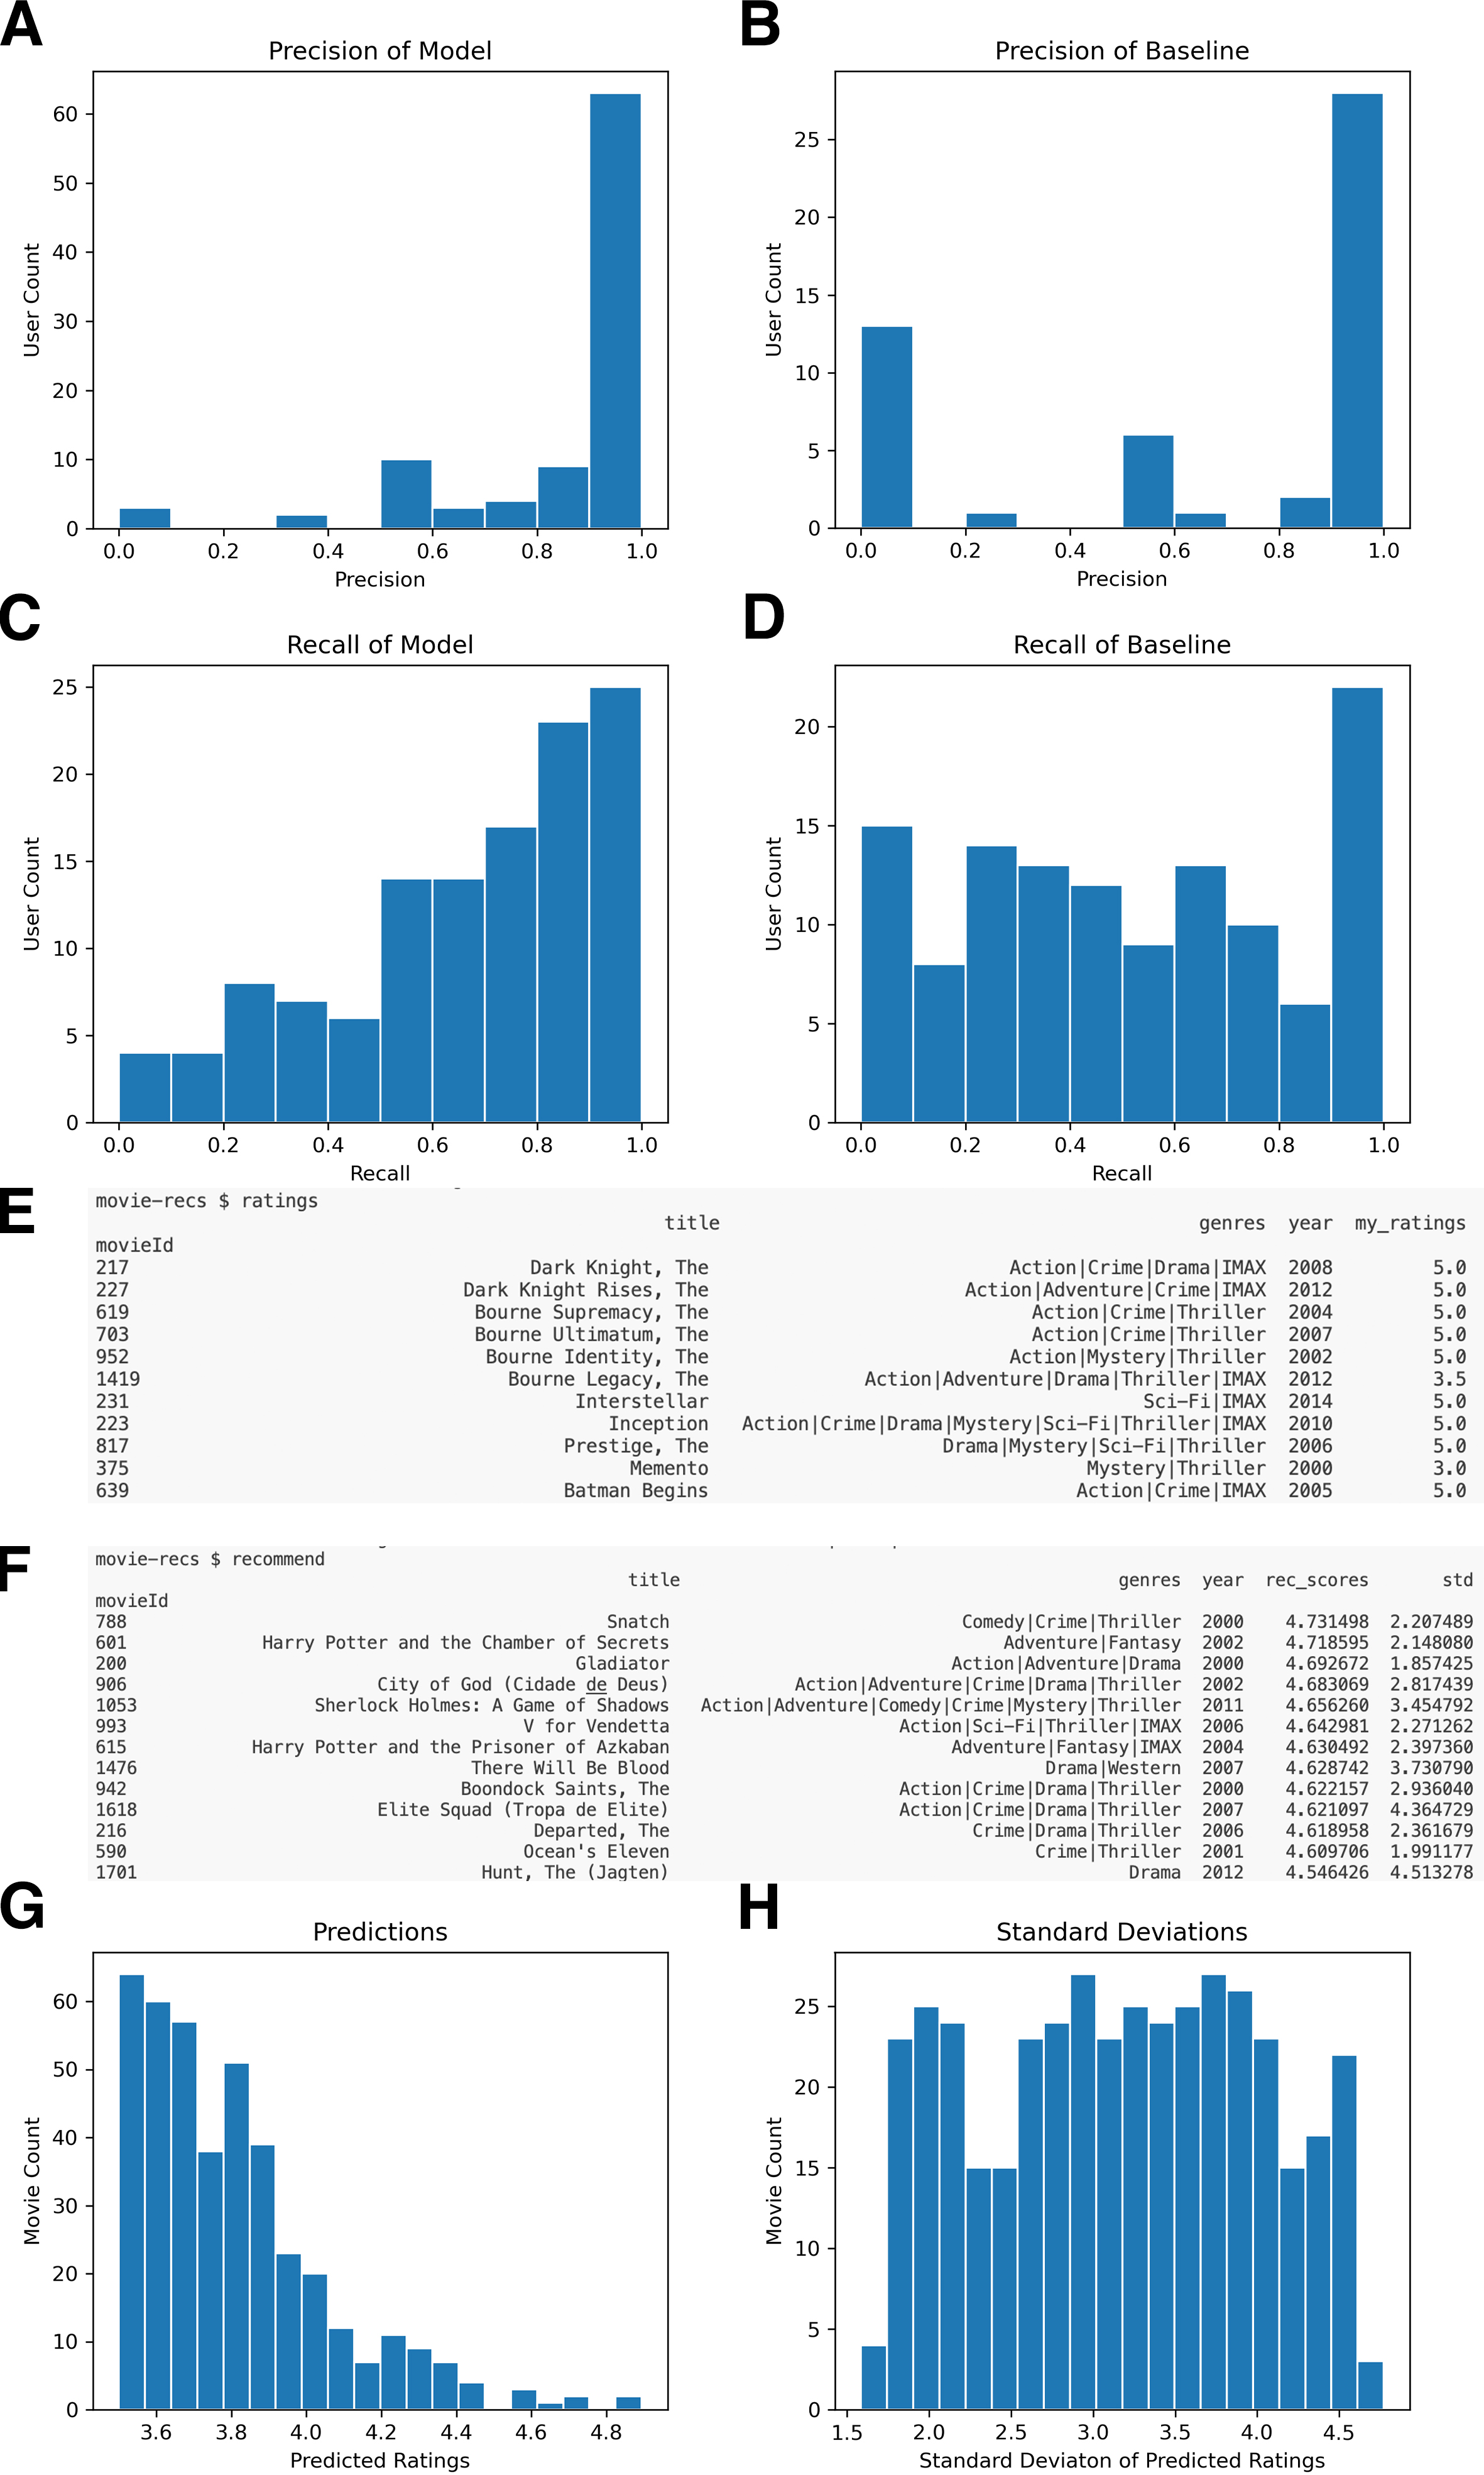
\includegraphics[width=0.75\textwidth]{inference.jpg}
    \caption{Inference using partial PMF. (A-D) Distribution of precision and recall of our model and baseline, which randomly suggests recommendations. (E-F) Given ratings as input into predictor and recommendation results. (G-H) Distribution of predicted ratings and standard deviations.}
    \label{fig:inference}
\end{figure}

\subsection{Analysis}

\begin{table}[H]
    \centering
    \caption{Performance of the recommendation model under different input sizes and the random control baseline.}
    \label{tab:results}
    \begin{tabular}{cccccc}
        \toprule
        \textbf{Input Size} & \textbf{Precision} & \textbf{Recall} & \textbf{F1-Score} & \textbf{MAE}    & \textbf{Baseline (Random)}                    \\
        \midrule
        0.1                 & \textbf{0.9069}    & 0.6137          & 0.7320            & 0.5884          & Precision: 0.6344, Recall: 0.4035, MAE: 1.326 \\
        0.3                 & 0.8631             & 0.7126          & 0.7807            & 0.6065          & Precision: 0.6325, Recall: 0.4550, MAE: 1.346 \\
        0.5                 & 0.8591             & 0.7124          & 0.7789            & 0.5943          & Precision: 0.7959, Recall: 0.4382, MAE: 1.123 \\
        0.7                 & 0.8836             & 0.7381          & \textbf{0.8043}   & \textbf{0.5399} & Precision: 0.7692, Recall: 0.5163, MAE: 1.283 \\
        0.9                 & 0.8788             & \textbf{0.7413} & 0.8042            & 0.5645          & Precision: 0.7573, Recall: 0.7413, MAE: 1.167 \\
        \bottomrule
    \end{tabular}
\end{table}

The results in Table~\ref{tab:results} show that our recommendation model consistently outperforms the random control baseline across all metrics. Key observations include:

\begin{itemize}
    \item Precision: The model achieves high precision values (above 0.85), indicating that most of the recommended movies are relevant to the user. In contrast, the random control baseline performs poorly, with precision values below 0.8.

    \item Recall: The recall values improve with larger input sizes, demonstrating that the model is able to capture a greater proportion of relevant movies when more user ratings are available.

    \item F1-Score: The harmonic mean of precision and recall reflects the overall performance of the model. The F1-Score reaches maximum when input size is 0.7, indicating a balanced improvement in precision and recall.

    \item MAE: The Mean Absolute Error is much lower compared to the baseline, highlighting the model's improved ability to predict user ratings more accurately with more input data.

\end{itemize}

Overall, the results demonstrate that our recommendation model provides accurate and comprehensive recommendations, with performance improving as more input data becomes available.

\section{Future Work}
For potential future work, there are multiple directions:
\begin{itemize}
    \item Algorithmic improvements: Currently, the model predicts missing ratings by fixing the movie feature matrix \(V\) and solving for the feature vector \(\vec{u}\) of the new user to approximate \(\vec{r} \approx V \vec{u}\). However, this approach disregards the information embedded in \(U\) obtained during the training process. Developing an algorithm that uses both \(U\) and \(V\) more effectively during the prediction phase could significantly improve recommendation accuracy.

    \item Larger datasets: Due to computational constraints, this project was limited to the MovieLens 100K dataset. Future work could explore the model's performance on larger datasets supplying more information potentially leading to improved prediction capabilities.

    \item Optimization of hyperparameters: While the current model uses a fixed set of hyperparameters, systematic optimization techniques such as grid search or random search would be used to fine-tune parameters like \(\lambda_U\), \(\lambda_V\), \(D\), and the learning rate \(\eta\). An adaptive learning rate could also be implemented to optimize the rate of convergence.

    \item Incorporating additional information: Our current model relies only on user ratings. Incorporating other information such as user demographics, movie genres, or metadata could supply more information for the latent representations and lead to more correctly personalized recommendations for the users.

    \item Evaluation metrics: Expanding the range of evaluation metrics to include measures such as Area Under the Curve (AUC) could provide a more complete assessment of the quality of the model's recommendations.

    \item Online learning: We can also extend the model to support real-time updates and recommendations based on streaming data. As new user ratings or interactions are received, the model updates $U$ and $V$ based on new user ratings.

\end{itemize}
By addressing these areas, the recommendation system can be further improved to deliver more accurate and user-centric recommendations.

\bibliographystyle{apacite}
\bibliography{references.bib}
\end{document}
